\chapter{Equilibrium Constants and Shifts}\label{ch:b2:equilibrium-shifts}

An ammonia plant runs its converter at about \qty{450}{\celsius} and
\qty{200}{bar}. At room temperature the equilibrium of \ce{N2 + 3H2 <=>
2NH3} lies so far towards ammonia that a mixture of the elements could in
principle be almost completely converted; yet the engineers heat it, which
pushes the equilibrium back, and then compress it to two hundred
atmospheres, which costs a great deal of energy. The reasons are a
compromise between how far a reaction can go and how fast it goes. This
chapter turns the \omterm{def:b2:reaction-free-energy:gibbs-energy}{Gibbs energy} of the previous chapters into the
equilibrium constant of the Year 1 volume, shows how that constant changes
with temperature, counts how many conditions an experimenter may choose
freely, and predicts in which direction an equilibrium moves when the
temperature, the pressure or the composition is changed.

\begin{recall}
\Cref{ch:b2:reaction-free-energy}: the evolution criterion $\Delta_r G\,\dd\xi
\leq 0$ and the Gibbs--Helmholtz relation;
\cref{ch:b2:chemical-potential}: $\Delta_r G = \Delta_r G^\circ + RT\ln Q$.
The Year 1 volume: the quotient $Q = \prod_i a_i^{\nu_i}$, the standard
equilibrium constant $K^\circ$ as the value of $Q$ at equilibrium, the law of
mass action and the rule ``$Q < K^\circ$: forward'', all stated there as
laws; progress tables; final states of one or two reactions. It also
promised that the choice of temperature and pressure for ammonia and for
sulfur trioxide would be explained here.
\end{recall}

\begin{omfigure}
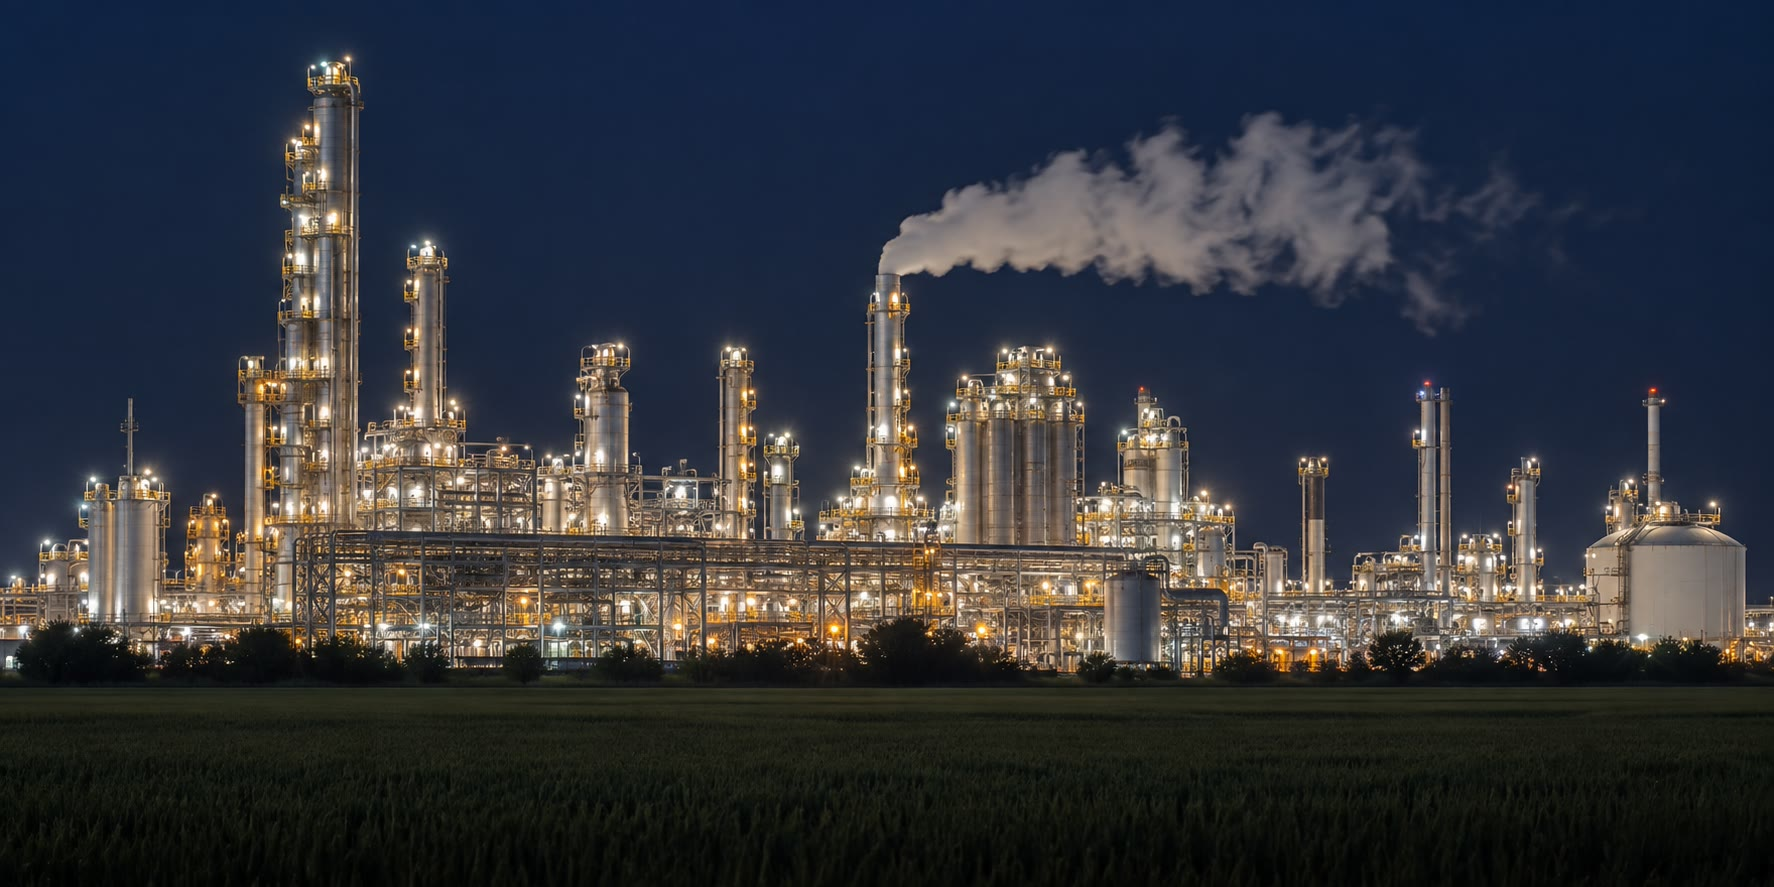
\includegraphics[width=0.7\linewidth]{images/book3/ai/b2-04-ammonia-plant.jpg}

{\small An ammonia plant at night. In its converter, nitrogen and hydrogen
pass over an iron catalyst at a few hundred degrees and a few hundred bar;
the choice of those conditions is the subject of the weekend problem.}
\end{omfigure}

\section{The equilibrium constant from the Gibbs energy}

\begin{theorem}[Standard equilibrium constant]\label{thm:b2:equilibrium-shifts:k-from-g}
At equilibrium $\Delta_r G = 0$, and the reaction quotient takes the value
\[
  K^\circ(T) = \exp\!\left(-\frac{\Delta_r G^\circ(T)}{RT}\right), \qquad
  \Delta_r G^\circ(T) = -RT\ln K^\circ(T) .
\]
It depends on the temperature alone.
\end{theorem}

\begin{proof}
The evolution criterion makes $\Delta_r G = 0$ the condition of equilibrium.
With $\Delta_r G = \Delta_r G^\circ + RT\ln Q$
(\cref{prop:b2:chemical-potential:delta-g-q}), equilibrium means $\ln Q_{\text{eq}}
= -\Delta_r G^\circ/(RT)$, a function of $T$ only since $\Delta_r G^\circ$ is.
\end{proof}

\begin{corollary}[The laws of the Year 1 volume]\label{cor:b2:equilibrium-shifts:mass-action}
$\Delta_r G = RT\ln(Q/K^\circ)$. Hence a system with $Q < K^\circ$ evolves
forward, one with $Q > K^\circ$ backward, and one with $Q = K^\circ$ is at
equilibrium (the law of mass action).
\end{corollary}

\begin{proof}
Substitute $\Delta_r G^\circ = -RT\ln K^\circ$ in $\Delta_r G = \Delta_r G^\circ
+ RT\ln Q$; the sign of $\Delta_r G$ is that of $\ln(Q/K^\circ)$, and the
evolution criterion requires $\Delta_r G\,\dd\xi \leq 0$.
\end{proof}

\begin{example}[Three constants at \qty{298}{K}]\label{ex:b2:equilibrium-shifts:constants}
Ammonia synthesis, $\Delta_r G^\circ = \qty{-32.8}{kJ/mol}$: $K^\circ =
\exp(32\,800/(8.314 \times 298.15)) = \num{5.6e5}$ (the tables, with more
digits, give \num{5.4e5}). The dissociation of \ce{N2O4}, $\Delta_r G^\circ =
\qty{+4.7}{kJ/mol}$: $K^\circ = 0.15$. The decomposition of limestone,
$\Delta_r G^\circ = \qty{+130.4}{kJ/mol}$: $K^\circ = \num{1.5e-23}$, and the
equilibrium pressure of carbon dioxide above limestone at room temperature
is $\num{1.5e-23}$ bar, nothing at all. A change of \qty{5.7}{kJ/mol} in
$\Delta_r G^\circ$ at \qty{298}{K} multiplies or divides $K^\circ$ by ten.
% ledger: dfh:NH3_g, s0:NH3_g, janafG:NH3.298.15 (computed in figdata/bachelor-2/thermo-data.py and vant-hoff.py)
\end{example}

The \omterm{def:b2:reaction-free-energy:gibbs-energy}{Gibbs energy} of the whole system shows the same thing as a landscape:
it is lowest at the equilibrium extent, where its slope, $\Delta_r G$, is
zero.

\begin{omfigure}
\begin{tikzpicture}
\begin{axis}[
  width=0.7\linewidth, height=5.6cm, xmin=0, xmax=1, ymin=-2.2, ymax=5.2,
  axis x line=bottom, axis y line=left, xlabel={extent $\xi$ (mol)},
  ylabel={$G(\xi) - G(0)$ (\unit{kJ})},
  tick label style={font=\small}, label style={font=\small}, clip=false]
\addplot[omDef, very thick] table[x=xi, y=G] {figdata/out/bachelor-2-gibbs-extent.dat};
\draw[dotted] (axis cs:0.189,-2.2) -- (axis cs:0.189,-0.949);
\fill[omThm] (axis cs:0.189,-0.949) circle (1.6pt);
\node[omThm, anchor=west, font=\small] at (axis cs:0.21,-1.75) {equilibrium, $\xi = 0.189$};
\draw[dashed, gray] (axis cs:0,0) -- (axis cs:1,4.728);
\node[gray, font=\scriptsize, anchor=south east] at (axis cs:1,4.75) {$\xi\,\Delta_r G^\circ$};
\end{axis}
\end{tikzpicture}

{\small \omterm{def:b2:reaction-free-energy:gibbs-energy}{Gibbs energy} of a closed system of perfect gases at \qty{298}{K} and
\qty{1}{bar}, starting from \qty{1}{mol} of \ce{N2O4}, against the extent of
\ce{N2O4 <=> 2NO2}. Although $\Delta_r G^\circ > 0$ (dashed line, pure
species), mixing the two gases lowers $G$, and the minimum lies at $\xi =
0.189$, where $Q = K^\circ = 0.15$. To its left the slope $\Delta_r G =
\partial G/\partial\xi$ is negative, to its right positive.}
% ledger: dfh:N2O4_g, s0:N2O4_g, dfh:NO2_g, s0:NO2_g (computed in figdata/bachelor-2/gibbs-extent.py)
\end{omfigure}

\section{Temperature: the van 't Hoff equation}

\begin{theorem}[van 't Hoff equation]\label{thm:b2:equilibrium-shifts:vant-hoff}
\[
  \frac{\dd\ln K^\circ}{\dd T} = \frac{\Delta_r H^\circ(T)}{RT^2}
\]
(the \emph{van 't Hoff equation}\index{van 't Hoff equation}): the equilibrium
constant of an \omterm{def:b2:reaction-enthalpy:exothermic}{endothermic} reaction increases with the temperature, that of
an \omterm{def:b2:reaction-enthalpy:exothermic}{exothermic} reaction decreases.
\end{theorem}

\begin{proof}
Write $\ln K^\circ = -\Delta_r G^\circ/(RT)$ and use the Gibbs--Helmholtz
relation of \cref{prop:b2:reaction-free-energy:gibbs-helmholtz},
\[
  \frac{\dd}{\dd T}\left(\frac{\Delta_r G^\circ}{T}\right) =
  -\frac{\Delta_r H^\circ}{T^2} ;
\]
divide by $-R$.
\end{proof}

\begin{proposition}[Integrated form]\label{prop:b2:equilibrium-shifts:integrated}
If $\Delta_r H^\circ$ is constant between $T_1$ and $T_2$ (\omterm{def:b2:reaction-free-energy:ellingham-approximation}{Ellingham
approximation}),
\[
  \ln\frac{K^\circ(T_2)}{K^\circ(T_1)} = -\frac{\Delta_r H^\circ}{R}\left(
  \frac{1}{T_2} - \frac{1}{T_1}\right),
\]
and $\ln K^\circ$ is a straight line of slope $-\Delta_r H^\circ/R$ against
$1/T$.
\end{proposition}

\begin{proof}
Integrate $\dd\ln K^\circ = (\Delta_r H^\circ/R)\,\dd T/T^2$, noting that
$\dd T/T^2 = -\dd(1/T)$.
\end{proof}

\begin{omfigure}
\begin{tikzpicture}
\begin{axis}[
  width=0.72\linewidth, height=5.8cm, xmin=0.9, xmax=3.5, ymin=-19, ymax=15,
  axis x line=bottom, axis y line=left, xlabel={$1000/T$ (\unit{1/K})},
  ylabel={$\ln K^\circ$}, tick label style={font=\small},
  label style={font=\small}, clip=false]
\addplot[omThm, dashed, thick] table[x=invT, y=lnK] {figdata/out/bachelor-2-vant-hoff-a-line.dat};
\addplot[omDef, only marks, mark=*, mark size=1.8pt] table[x=invT, y=lnK] {figdata/out/bachelor-2-vant-hoff-a.dat};
\node[omDef, font=\scriptsize, anchor=west] at (axis cs:3.36,13.2) {\qty{298}{K}};
\node[omDef, font=\scriptsize, anchor=north west] at (axis cs:1.03,-15.3) {\qty{1000}{K}};
\node[omThm, font=\small, anchor=south east, align=right] at (axis cs:2.4,8) {slope $-\Delta_r H^\circ(298)/R$\\ $= +11\,050$ K};
\end{axis}
\end{tikzpicture}

{\small The constant of \ce{N2 + 3H2 <=> 2NH3} from the tables (dots, 298 to
\qty{1000}{K}) and the van 't Hoff line drawn with $\Delta_r H^\circ$ at
\qty{298}{K} (dashed). The reaction is \omterm{def:b2:reaction-enthalpy:exothermic}{exothermic}: $K^\circ$ falls from
\num{5e5} to \num{3e-7}. At high temperature the dots fall below the line:
$\Delta_r H^\circ$ becomes more negative as $T$ rises
(\cref{ex:b2:reaction-enthalpy:kirchhoff}).}
% ledger: janafG:NH3.298.15, janafG:NH3.400, janafG:NH3.500, janafG:NH3.600, janafG:NH3.700, janafG:NH3.800, janafG:NH3.900, janafG:NH3.1000, dfh:NH3_g (computed in figdata/bachelor-2/vant-hoff.py)
\end{omfigure}

\begin{method}[An equilibrium constant at another temperature]\label{met:b2:equilibrium-shifts:k-at-t}
\begin{enumerate}
  \item From tables at \qty{298}{K}, compute $\Delta_r H^\circ$, $\Delta_r
        S^\circ$, and $K^\circ(298)$.
  \item Either use the integrated \omterm{thm:b2:equilibrium-shifts:vant-hoff}{van 't Hoff equation}, or compute
        $\Delta_r G^\circ(T) = \Delta_r H^\circ - T\Delta_r S^\circ$ and then
        $K^\circ(T)$: the two are the same approximation.
  \item For a wide interval or a large $\Delta_r C_p^\circ$, prefer tabulated
        $\Delta_f G^\circ(T)$; an error of \qty{5.7}{kJ/mol} at \qty{298}{K}
        (or \qty{13}{kJ/mol} at \qty{700}{K}) is a factor of ten on $K^\circ$.
\end{enumerate}
\end{method}

\begin{history}[Jacobus Henricus van 't Hoff]
\begin{minipage}[t]{0.2\linewidth}\vspace{0pt}
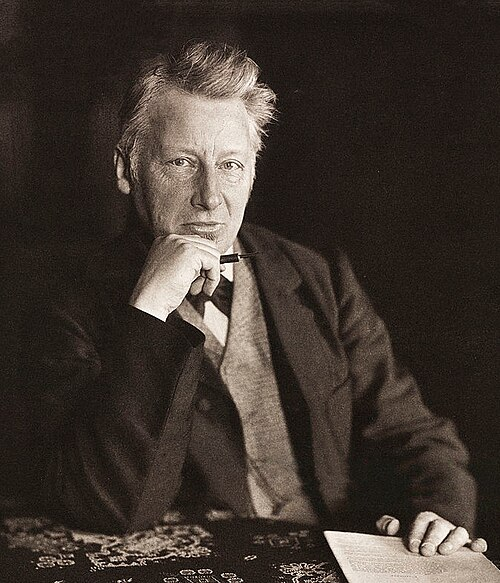
\includegraphics[width=\linewidth]{images/book3/vanthoff.jpg}
\end{minipage}\hfill
\begin{minipage}[t]{0.76\linewidth}\vspace{0pt}
Jacobus Henricus van 't Hoff (1852--1911) gave in 1884, in his
\emph{Studies in Chemical Dynamics}, the relation between the temperature and
the equilibrium constant that bears his name, and the next year the law of
\omterm{def:b2:chemical-potential:osmotic-pressure}{osmotic pressure} of \cref{ch:b2:chemical-potential}; ten years earlier he had
proposed the tetrahedral carbon atom. He received the first Nobel Prize in
Chemistry, in 1901. (Photograph by N. Perscheid, 1904: public domain,
Wikimedia Commons.)
\end{minipage}
\end{history}

\section{Variance}

How many intensive quantities can an experimenter fix freely before the
equilibrium state is completely determined?

\begin{definition}[Variance]\label{def:b2:equilibrium-shifts:variance}
The \emph{independent intensive parameters}\index{independent intensive parameter}
of a system at equilibrium are a set of intensive quantities
(temperature, pressure, mole fractions in each phase) that can be chosen
independently and that, once chosen, fix all the others. Their number is the
\emph{variance}\index{variance} $v$ of the system.
\end{definition}

\begin{theorem}[Phase rule]\label{thm:b2:equilibrium-shifts:phase-rule}
For a system of $n$ species distributed among $\varphi$ phases, linked by $r$
independent equilibrium reactions and $s$ additional relations between
intensive quantities fixed by the preparation (a stoichiometric feed,
electroneutrality),
\[
  v = c + 2 - \varphi, \qquad c = n - r - s .
\]
\end{theorem}

\begin{proof}
Intensive variables: $T$, $p$, and in each phase the mole fractions of the
$n$ species, which sum to 1, so $n - 1$ free ones per phase: in all $2 +
\varphi(n - 1)$. Relations: each species is at equilibrium between the
phases, $\varphi - 1$ equalities of \omterm{def:b2:chemical-potential:chemical-potential}{chemical potentials} per species, $n(\varphi -
1)$ in all; each reaction gives $Q = K^\circ(T)$, $r$ relations; and $s$
additional relations. Subtract: $v = 2 + \varphi(n - 1) - n(\varphi - 1) - r -
s = n - r - s + 2 - \varphi$. (A species absent from a phase removes one
variable and one relation together.)
\end{proof}

\begin{method}[Computing a variance]\label{met:b2:equilibrium-shifts:variance}
\begin{enumerate}
  \item List the species, with their phase, and count $n$ and $\varphi$
        (each pure solid is a phase; all gases form one phase).
  \item Count the independent reactions $r$ among them.
  \item Count the extra relations $s$: amounts in stoichiometric proportion
        (only if the relation is between quantities of the same phase),
        electroneutrality of an ionic solution.
  \item $v = n - r - s + 2 - \varphi$.
\end{enumerate}
\end{method}

\begin{example}[Three variances]\label{ex:b2:equilibrium-shifts:variances}
Limestone in a closed vessel, \ce{CaCO3(s) <=> CaO(s) + CO2(g)}: $n = 3$, $r =
1$, $\varphi = 3$ (two solids, one gas): $v = 1$. Choose $T$, and the pressure
of carbon dioxide is fixed: $p = K^\circ(T)\,p^\circ$. A gas mixture of
\ce{N2}, \ce{H2} and \ce{NH3} at equilibrium: $n = 3$, $r = 1$, $\varphi = 1$, $v
= 3$ ($T$, $p$ and one composition variable); made from ammonia alone, or from
a stoichiometric feed, \ce{N2} and \ce{H2} are in the ratio 1 : 3, $s = 1$ and
$v = 2$: at given $T$ and $p$ the composition is fixed, as the weekend problem
uses.
\end{example}

\section{Shifting an equilibrium}

\begin{definition}[Shift of an equilibrium]\label{def:b2:equilibrium-shifts:shift}
When a system at equilibrium is perturbed (a change of temperature, of
pressure, or of an amount), it is no longer at equilibrium in general and
evolves to a new one. The \emph{shift of the equilibrium}\index{shift of an equilibrium}
is forward if the reaction advances ($\dd\xi > 0$) and backward
otherwise.
\end{definition}

\begin{method}[Predicting a shift]\label{met:b2:equilibrium-shifts:predict-shift}
Just after the perturbation, compute (or estimate the sign of the change of)
$Q$ and $K^\circ$. If now $Q < K^\circ$, the shift is forward; if $Q > K^\circ$,
backward; if the equality still holds, there is no shift.
\end{method}

\begin{omfigure}
\begin{tikzpicture}[font=\small, >={Stealth}]
  \draw[->, thick] (0,0) -- (11,0) node[right] {$\ln Q$};
  \draw[omThm, thick] (5.5,0.25) -- (5.5,-0.25) node[below, align=center] {$\ln K^\circ$\\ ($= \ln Q$ before)};
  \fill (5.5,0) circle (2pt);
  \draw[omDef, thick] (2.8,0.25) -- (2.8,-0.25) node[below] {$\ln Q$ just after};
  \draw[->, omDef, very thick] (3.0,0.6) -- (5.2,0.6) node[midway, above] {forward shift};
  \draw[omProp, thick] (8.4,0.25) -- (8.4,-0.25) node[below] {$\ln Q$ just after};
  \draw[->, omProp, very thick] (8.2,0.6) -- (5.8,0.6) node[midway, above] {backward shift};
\end{tikzpicture}

{\small A perturbation moves $Q$ (or $K^\circ$, if the temperature changes);
the system then shifts until $Q = K^\circ$ again, forward if $Q$ has become
too small, backward if too large.}
\end{omfigure}

\begin{proposition}[Temperature]\label{prop:b2:equilibrium-shifts:temperature}
At constant pressure, raising the temperature shifts an equilibrium in the
\omterm{def:b2:reaction-enthalpy:exothermic}{endothermic} direction (forward if $\Delta_r H^\circ > 0$), lowering it in the
\omterm{def:b2:reaction-enthalpy:exothermic}{exothermic} direction.
\end{proposition}

\begin{proof}
At fixed composition and pressure, $Q$ does not change with $T$ (for ideal
systems); by van 't Hoff, $K^\circ$ increases with $T$ if $\Delta_r H^\circ >
0$. Just after a rise of $T$, then, $Q < K^\circ$: forward.
\end{proof}

\begin{proposition}[Pressure]\label{prop:b2:equilibrium-shifts:pressure}
At constant temperature and composition, raising the total pressure of a
gas-phase equilibrium shifts it in the direction that lowers the number of
gas molecules ($\Delta\nu_{\text{gas}} < 0$ forward). If $\Delta\nu_{\text{gas}}
= 0$, the pressure has no effect.
\end{proposition}

\begin{proof}
With $p_i = x_ip$, $Q = \prod_i x_i^{\nu_i}\,(p/p^\circ)^{\Delta\nu_{\text{gas}}}$:
at fixed composition, raising $p$ multiplies $Q$ by
$(p'/p)^{\Delta\nu_{\text{gas}}}$, which is $< 1$ if $\Delta\nu_{\text{gas}} <
0$. Then $Q < K^\circ$: forward. Condensed phases contribute nothing.
\end{proof}

\begin{proposition}[Adding a constituent or an inert gas]\label{prop:b2:equilibrium-shifts:adding}
Adding a small amount of a gaseous constituent $j$ to a gas-phase equilibrium
changes $\ln Q$ by
\[
  \left(\frac{\partial\ln Q}{\partial n_j}\right) = \frac{\nu_j}{n_j} -
  \frac{\Delta\nu_{\text{gas}}}{n_{\text{tot}}}\ \ \text{at constant } T, p ;
  \qquad \frac{\nu_j}{n_j}\ \ \text{at constant } T, V .
\]
Adding an inert gas has no effect at constant volume, and at constant pressure
acts as a lowering of the pressure.
\end{proposition}

\begin{proof}
At constant $T$, $p$: $Q = \prod_i n_i^{\nu_i}\,(p/(p^\circ n_{\text{tot}}))^{
\Delta\nu_{\text{gas}}}$, whose logarithmic derivative with respect to $n_j$ is
$\nu_j/n_j - \Delta\nu_{\text{gas}}/n_{\text{tot}}$ (zero first term for an inert
gas, $\nu_j = 0$). At constant $T$, $V$: $p_i = n_iRT/V$ and $Q = \prod_i n_i^{
\nu_i}\,(RT/(p^\circ V))^{\Delta\nu_{\text{gas}}}$, whose derivative is
$\nu_j/n_j$ alone.
\end{proof}

\begin{remark}[A reactant added that drives the reaction backward]\label{rem:b2:equilibrium-shifts:paradox}
In ammonia synthesis, $\nu(\ce{N2}) = -1$ and $\Delta\nu_{\text{gas}} = -2$:
adding nitrogen at constant $T$ and $p$ changes $\ln Q$ by $-1/n_{\ce{N2}} +
2/n_{\text{tot}}$, which is positive when $x(\ce{N2}) > 1/2$. In a mixture
already rich in nitrogen, adding more nitrogen dilutes the hydrogen so much
that ammonia decomposes. The rule ``adding a reactant pushes forward'' is safe
at constant volume, not always at constant pressure.
\end{remark}

\begin{proposition}[Le Chatelier's principle]\label{prop:b2:equilibrium-shifts:le-chatelier}
The propositions above are summed up by \emph{Le Chatelier's
principle}\index{Le Chatelier's principle}: a system at equilibrium,
perturbed in temperature or pressure, shifts in the direction that opposes
the perturbation (it absorbs heat when heated, reduces its gas volume when
compressed).
\end{proposition}

\begin{proof}
It restates \cref{prop:b2:equilibrium-shifts:temperature} (the \omterm{def:b2:reaction-enthalpy:exothermic}{endothermic}
direction absorbs heat) and \cref{prop:b2:equilibrium-shifts:pressure} (fewer
gas molecules occupy less volume at the same $T$ and $p$). For additions of
matter at constant pressure the principle is not reliable
(\cref{rem:b2:equilibrium-shifts:paradox}): compute $Q$.
\end{proof}

\begin{remark}[When the equilibrium ends]\label{rem:b2:equilibrium-shifts:rupture}
A shift can end not in a new equilibrium but in the disappearance of a phase.
Heated in a closed vessel, limestone decomposes until $p(\ce{CO2}) =
K^\circ(T)\,p^\circ$; if there is not enough of it to reach that pressure, it
disappears entirely and $Q$ stays below $K^\circ$: the system is out of
equilibrium for good, as the Year 1 volume already observed.
\end{remark}

\begin{history}[Henry Le Chatelier]
\begin{minipage}[t]{0.2\linewidth}\vspace{0pt}
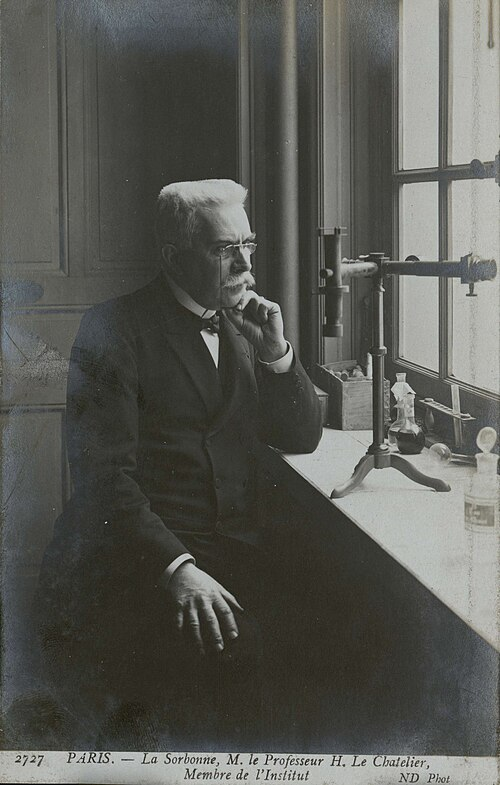
\includegraphics[width=\linewidth]{images/book3/lechatelier.jpg}
\end{minipage}\hfill
\begin{minipage}[t]{0.76\linewidth}\vspace{0pt}
Henry Le Chatelier (1850--1936), a mining engineer and chemist who worked on
cements, metallurgy and pyrometry, stated in 1884 the ``law of displacement
of equilibrium'' named after him. He had also tried, around 1901, to make
ammonia from its elements under pressure; an explosion in his apparatus ended
the attempt. (Photograph: unknown author, CC BY-SA 4.0, Wikimedia Commons.)
\end{minipage}
\end{history}

\section{Optimising a synthesis}

\subsection*{Ammonia}

\begin{omfigure}
\begin{tikzpicture}
\begin{axis}[
  width=0.78\linewidth, height=6.2cm, xmin=500, xmax=1000, ymin=0, ymax=0.9,
  axis x line=bottom, axis y line=left, xlabel={$T$ (K)},
  ylabel={equilibrium mole fraction of \ce{NH3}},
  tick label style={font=\small}, label style={font=\small}, clip=false]
\addplot[omThm, very thick] table[x=T, y=p300] {figdata/out/bachelor-2-vant-hoff-b.dat};
\addplot[omDef, very thick] table[x=T, y=p200] {figdata/out/bachelor-2-vant-hoff-b.dat};
\addplot[omProp, very thick] table[x=T, y=p50] {figdata/out/bachelor-2-vant-hoff-b.dat};
\addplot[black!60, very thick] table[x=T, y=p1] {figdata/out/bachelor-2-vant-hoff-b.dat};
\node[omThm, font=\scriptsize, anchor=south west] at (axis cs:600,0.70) {300 bar};
\node[omDef, font=\scriptsize, anchor=north east] at (axis cs:612,0.52) {200 bar};
\node[omProp, font=\scriptsize, anchor=north east] at (axis cs:578,0.30) {50 bar};
\node[black!60, font=\scriptsize, anchor=south west] (onebar) at (axis cs:520,0.13) {1 bar};
\draw[black!60] (onebar.south west) -- (axis cs:512,0.075);
\draw[dotted] (axis cs:723,0) -- (axis cs:723,0.253);
\fill[omDef] (axis cs:723,0.253) circle (1.6pt);
\end{axis}
\end{tikzpicture}

{\small Equilibrium mole fraction of ammonia from a 1 : 3 mixture of nitrogen
and hydrogen (perfect gases), against temperature at four pressures,
computed from the tabulated Gibbs energies. Pressure raises it, temperature
lowers it; the dot marks \qty{723}{K} and \qty{200}{bar}.}
% ledger: janafG:NH3.500, janafG:NH3.600, janafG:NH3.700, janafG:NH3.800, janafG:NH3.900, janafG:NH3.1000 (computed in figdata/bachelor-2/vant-hoff.py)
\end{omfigure}

The synthesis is \omterm{def:b2:reaction-enthalpy:exothermic}{exothermic} and reduces four molecules of gas to two: by
the propositions above, low temperature and high pressure favour ammonia.
At \qty{1}{bar} and room temperature the equilibrium is almost complete, but
the reaction does not run at all: the triple bond of nitrogen is broken only
on a catalyst, and the iron catalyst works only at several hundred
degrees. Plants therefore choose:
\begin{itemize}
  \item a temperature high enough for the rate, as low as the catalyst allows
        (around \qty{700}{K});
  \item a high pressure to recover the yield lost to the temperature, limited
        by the cost of compression and of thick-walled vessels;
  \item a loop: the gas leaving the converter is cooled, the ammonia condenses
        and is removed, and the unconverted gas is recycled with fresh feed;
        a small \omterm{def:b2:equilibrium-shifts:single-pass}{purge} removes the argon and methane that would otherwise
        accumulate.
\end{itemize}

\begin{definition}[Single-pass conversion, recycle, purge]\label{def:b2:equilibrium-shifts:single-pass}
In a process with recycling, the \emph{single-pass conversion}\index{single-pass conversion}
is the fraction of a reactant converted in one passage through
the reactor; the unconverted part, separated from the product, is returned
to the reactor inlet as the \emph{recycle}\index{recycle}; a
\emph{purge}\index{purge} is a small stream withdrawn continuously from the
recycle to keep inert species from accumulating.
\end{definition}

\begin{omfigure}
\begin{tikzpicture}[font=\small, >={Stealth}, box/.style={draw, thick, rounded corners=2pt, minimum width=2.1cm, minimum height=1.0cm, align=center, fill=white}]
  \node[box] (comp) at (0,0) {compressor};
  \node[box] (conv) at (3.6,0) {converter\\ (catalyst)};
  \node[box] (cond) at (7.2,0) {cooler and\\ separator};
  \draw[->, thick] (-3.9,0) -- (comp) node[pos=0.0, above right] {fresh \ce{N2 + 3H2}};
  \draw[->, thick] (comp) -- (conv);
  \draw[->, thick] (conv) -- (cond);
  \draw[->, thick, omDef] (cond.south) -- ++(0,-1.0) node[below] {liquid ammonia};
  \draw[->, thick, omThm] (cond.north) -- ++(0,0.9) -| (comp.north);
  \node[omThm, above] at (2.6,1.4) {recycle (unconverted gas)};
  \draw[->, thick, black!60] (6.1,1.4) -- (6.1,2.1) node[above] {purge};
\end{tikzpicture}

{\small The ammonia loop. Each pass converts only part of the gas; ammonia
is condensed out, and the rest is recompressed and sent back with the fresh
feed. The \omterm{def:b2:equilibrium-shifts:single-pass}{purge} keeps argon and methane, which do not react, from building
up.}
\end{omfigure}

\begin{history}[Haber and Bosch]
\begin{minipage}[t]{0.15\linewidth}\vspace{0pt}
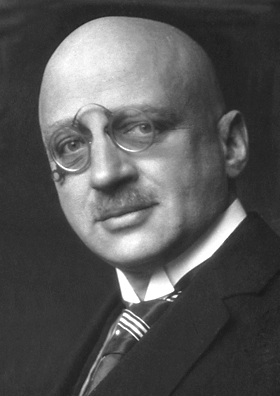
\includegraphics[width=\linewidth]{images/book3/haber.png}
\end{minipage}\hspace{0.01\linewidth}%
\begin{minipage}[t]{0.15\linewidth}\vspace{0pt}
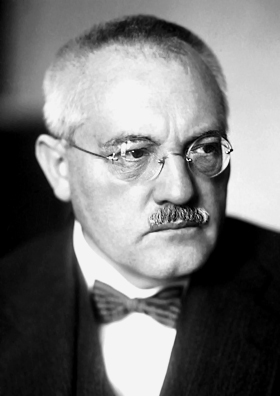
\includegraphics[width=\linewidth]{images/book3/bosch.jpg}
\end{minipage}\hfill
\begin{minipage}[t]{0.66\linewidth}\vspace{0pt}
Fritz Haber (1868--1934) measured the equilibrium of ammonia under pressure
and, in 1909, made it flow continuously from a laboratory converter over an
osmium catalyst. Carl Bosch (1874--1940) turned it into an industry, with
steel vessels that resisted hot hydrogen under pressure and a cheap iron
catalyst; the first plant started in 1913. Haber received the Nobel Prize in
1918, Bosch in 1931. (Nobel Foundation portraits: public domain, Wikimedia
Commons.)
\end{minipage}
\end{history}

\subsection*{Sulfur trioxide}

In the contact process, \ce{2SO2(g) + O2(g) <=> 2SO3(g)} ($\Delta_r H^\circ =
\qty{-197.8}{kJ/mol}$ for the equation as written) runs over a vanadium oxide
catalyst, active only when hot, in several adiabatic beds. In each bed the
heat released raises the temperature, which lowers $K^\circ$; the conversion
stops when the gas reaches the equilibrium curve. Cooling between beds brings
it back to a temperature where the equilibrium allows more conversion.
% ledger: dfh:SO2_g, dfh:SO3_g

\begin{omfigure}
\begin{tikzpicture}
\begin{axis}[
  width=0.72\linewidth, height=6.4cm, xmin=600, xmax=900, ymin=0, ymax=1.08,
  axis x line=bottom, axis y line=left, xlabel={$T$ (K)},
  ylabel={conversion of \ce{SO2}}, tick label style={font=\small},
  label style={font=\small}, clip=false]
\addplot[black, very thick] table[x=T, y=X] {figdata/out/bachelor-2-vant-hoff-c.dat};
\addplot[omThm, thick] table[x=T, y=X] {figdata/out/bachelor-2-vant-hoff-bed1.dat};
\addplot[omThm, thick] table[x=T, y=X] {figdata/out/bachelor-2-vant-hoff-bed2.dat};
\addplot[omThm, thick] table[x=T, y=X] {figdata/out/bachelor-2-vant-hoff-bed3.dat};
\draw[->, omDef, thick] (axis cs:892.8,0.676) -- (axis cs:712,0.676);
\draw[->, omDef, thick] (axis cs:784.4,0.924) -- (axis cs:712,0.924);
\node[font=\scriptsize, anchor=south west] at (axis cs:860,0.84) {equilibrium};
\node[omThm, font=\scriptsize, anchor=west] at (axis cs:800,0.24) {bed 1 (adiabatic)};
\node[omDef, font=\scriptsize, anchor=south] at (axis cs:800,0.68) {cooling};
\end{axis}
\end{tikzpicture}

{\small Equilibrium conversion of \ce{SO2} to \ce{SO3} against temperature
(black) for a model feed of \qty{10}{\percent} \ce{SO2}, \qty{11}{\percent}
\ce{O2} at \qty{1}{bar}, and the path of the gas through three adiabatic beds
(red, rising in temperature as the reaction heats the gas), cooled between
beds (blue).}
% ledger: janafG:SO2.600, janafG:SO2.700, janafG:SO2.800, janafG:SO2.900, janafG:SO3.600, janafG:SO3.700, janafG:SO3.800, janafG:SO3.900 (computed in figdata/bachelor-2/vant-hoff.py; feed and adiabatic rise are model values)
\end{omfigure}

\section{Exercises}

\begin{exercise}[$\star$]\label{exo:b2:equilibrium-shifts:1}
Compute $K^\circ$ at \qty{298}{K} for a reaction with $\Delta_r G^\circ =
\qty{-32.8}{kJ/mol}$, then for $\Delta_r G^\circ = \qty{+32.8}{kJ/mol}$.
What change of $\Delta_r G^\circ$ multiplies $K^\circ$ by 100?
\end{exercise}

\begin{exercise}[$\star$]\label{exo:b2:equilibrium-shifts:2}
For ammonia synthesis $K^\circ(298) = \num{5.4e5}$ and $\Delta_r H^\circ =
\qty{-91.9}{kJ/mol}$. Estimate $K^\circ$ at \qty{400}{K} with the integrated
\omterm{thm:b2:equilibrium-shifts:vant-hoff}{van 't Hoff equation}; the tables give 35.6.
\end{exercise}

\begin{exercise}[$\star$]\label{exo:b2:equilibrium-shifts:3}
Compute the \omterm{def:b2:equilibrium-shifts:variance}{variance} of: (a) liquid water in equilibrium with its vapour;
(b) \ce{CaCO3(s) <=> CaO(s) + CO2(g)} in a closed vessel; (c) \ce{N2},
\ce{H2}, \ce{NH3} at equilibrium, arbitrary feed; (d) \ce{C(s) + H2O(g) <=>
CO(g) + H2(g)}.
\end{exercise}

\begin{exercise}[$\star$]\label{exo:b2:equilibrium-shifts:4}
For \ce{N2O4(g) <=> 2NO2(g)}, $\Delta_r H^\circ > 0$. In which direction is the
equilibrium shifted by heating at constant pressure, by compressing at
constant temperature, by adding argon at constant volume?
\end{exercise}

\begin{exercise}[$\star\star$]\label{exo:b2:equilibrium-shifts:5}
For \ce{N2(g) + O2(g) <=> 2NO(g)}, $\Delta_r H^\circ = \qty{180.6}{kJ/mol}$,
$\Delta_r S^\circ = \qty{24.8}{J/(K.mol)}$. Compute $K^\circ$ at \qty{298}{K}
and at \qty{2000}{K} (\omterm{def:b2:reaction-free-energy:ellingham-approximation}{Ellingham approximation}), and the mole fraction of
\ce{NO} in air ($x(\ce{N2}) = 0.78$, $x(\ce{O2}) = 0.21$, little consumed) at
equilibrium at \qty{2000}{K}. Why do engines make this pollutant, and why
does it survive in the cooled exhaust?
\end{exercise}

\begin{exercise}[$\star\star$]\label{exo:b2:equilibrium-shifts:6}
An esterification $\mathrm{A + B \rightleftharpoons E + W}$ in the liquid phase
has $K^\circ = 4.0$ (activities taken as mole fractions). Starting from
\qty{1.0}{mol} of acid A, compute the amount of ester with \qty{1.0}{mol}, then
\qty{3.0}{mol} of alcohol B. Explain, with $Q$ and $K^\circ$, why removing the
water as it forms drives the reaction to completion.
\end{exercise}

\begin{exercise}[$\star\star$]\label{exo:b2:equilibrium-shifts:7}
At \qty{298}{K} and \qty{1}{bar}, $K^\circ = 0.148$ for \ce{N2O4 <=> 2NO2}.
Compute the degree of dissociation of \qty{1}{mol} of \ce{N2O4}. Then
\qty{1}{mol} of argon is added at constant total pressure: compute the new
degree of dissociation, and explain. What happens if the argon is added at
constant volume?
\end{exercise}

\begin{exercise}[$\star\star$]\label{exo:b2:equilibrium-shifts:8}
Ammonium chloride sublimes by dissociating, \ce{NH4Cl(s) <=> NH3(g) +
HCl(g)}. Compute the \omterm{def:b2:equilibrium-shifts:variance}{variance} when the gas is made only by the solid, and when
some ammonia has been added. What does each case mean for the experimenter?
\end{exercise}

\begin{exercise}[$\star\star$]\label{exo:b2:equilibrium-shifts:9}
The tables give, for ammonia synthesis, $K^\circ = 0.0993$ at \qty{500}{K} and
$K^\circ = \num{1.72e-3}$ at \qty{600}{K}. Deduce $\Delta_r H^\circ$ in that
interval and compare with its value at \qty{298}{K}.
\end{exercise}

\begin{exercise}[$\star\star\star$]\label{exo:b2:equilibrium-shifts:10}
Prove the counter-example of \cref{rem:b2:equilibrium-shifts:paradox}: write
$Q$ of ammonia synthesis with the amounts and the total pressure, compute
$\partial\ln Q/\partial n(\ce{N2})$ at constant $T$ and $p$, and find the
condition on $x(\ce{N2})$ for which adding nitrogen shifts the equilibrium
backward. Can the same happen at constant volume?
\end{exercise}

\begin{exercise}[$\star\star\star$]\label{exo:b2:equilibrium-shifts:11}
Limestone is heated to \qty{1100}{K} in an empty closed vessel of
\qty{10.0}{L}, where $\Delta_r G^\circ = \qty{1.62}{kJ/mol}$ for its
decomposition (\cref{ch:b2:reaction-free-energy}). Compute $K^\circ$ and the
equilibrium pressure of carbon dioxide. Find the final state for
\qty{0.050}{mol} and for \qty{0.200}{mol} of limestone.
\end{exercise}

\begin{exercise}[$\star\star\star$]\label{exo:b2:equilibrium-shifts:12}
Read on the contact-process figure the conversion and the temperature at the
outlet of each bed. Explain why a single adiabatic bed, however long, could
not exceed about 68\,\% conversion with this feed, why the gas is cooled
between beds rather than the catalyst kept cold throughout, and what limits
the conversion of the last bed.
\end{exercise}

\section{Problem: The Ammonia Loop}

\begin{problem}[{Weekend problem --- the equilibrium constant of ammonia
synthesis and its temperature dependence, the composition at the converter's
conditions, the shifts caused by pressure, temperature and inert gases, and
the loop}]
\label{pb:b2:equilibrium-shifts:1}
Ammonia is made by \ce{N2(g) + 3H2(g) <=> 2NH3(g)} from a stoichiometric feed.
Data: at \qty{298.15}{K}, $\Delta_f H^\circ(\ce{NH3}) = \qty{-45.94}{kJ/mol}$,
$S^\circ_m$ (\unit{J/(K.mol)}) \ce{NH3} 192.77, \ce{N2} 191.61, \ce{H2} 130.68;
the tables give $\Delta_f G^\circ(\ce{NH3}) = \qty{+27.19}{kJ/mol}$ at
\qty{700}{K} and \qty{+38.66}{kJ/mol} at \qty{800}{K}. Gases are perfect;
$R = \qty{8.314}{J/(K.mol)}$.
% ledger: dfh:NH3_g, s0:NH3_g, s0:N2_g, s0:H2_g, janafG:NH3.700, janafG:NH3.800

\medskip
\noindent\textbf{Part I --- The constant.}
\begin{enumerate}
  \item Compute $\Delta_r H^\circ$, $\Delta_r S^\circ$ and $\Delta_r G^\circ$ at
        \qty{298}{K}, and $K^\circ(298)$.
  \item Compute $K^\circ$ at \qty{700}{K} and at \qty{800}{K} from the tables.
  \item Deduce from these two values the mean $\Delta_r H^\circ$ between
        \qty{700}{K} and \qty{800}{K}, and compare with question 1.
  \item Estimate $K^\circ(\qty{723}{K})$ from the two tabulated values with
        the \omterm{thm:b2:equilibrium-shifts:vant-hoff}{van 't Hoff equation}.
  \item Compute $K^\circ(\qty{723}{K})$ in the \omterm{def:b2:reaction-free-energy:ellingham-approximation}{Ellingham approximation} from
        the data at \qty{298}{K}, and comment on the difference.
\end{enumerate}

\medskip
\noindent\textbf{Part II --- The equilibrium in the converter.}
\begin{enumerate}[resume]
  \item From a feed of \qty{1}{mol} \ce{N2} and \qty{3}{mol} \ce{H2}, write the
        amounts at extent $\xi$ and the total amount.
  \item Show that, with $x$ the mole fraction of ammonia, the mole fractions
        of \ce{N2} and \ce{H2} are $(1-x)/4$ and $3(1-x)/4$.
  \item Show that $\dfrac{x}{(1-x)^2} = \dfrac{\sqrt{27}}{16}\,\dfrac{p}{p^\circ}\,
        \sqrt{K^\circ}$.
  \item Compute $x$ at \qty{723}{K} and \qty{1}{bar}.
  \item Compute $x$ at \qty{723}{K} and \qty{200}{bar}.
  \item Compute the \omterm{def:b2:equilibrium-shifts:variance}{variance} of the system and explain why $T$ and $p$ fix the
        composition.
\end{enumerate}

\medskip
\noindent\textbf{Part III --- Shifts.}
\begin{enumerate}[resume]
  \item Without computing, in which direction does the equilibrium move when
        the pressure rises? When the temperature rises?
  \item Argon enters with the air used to make the nitrogen. At constant total
        pressure, how does its presence shift the equilibrium?
  \item A mixture at equilibrium has $x(\ce{N2}) = 0.30$. Does adding a little
        nitrogen at constant $T$ and $p$ shift it forward or backward?
  \item Would the answer change at constant volume?
  \item Before the gas returns to the converter, its ammonia is condensed
        out. What does this do to $Q$ at the converter inlet?
\end{enumerate}

\medskip
\noindent\textbf{Part IV --- The loop.}
\begin{enumerate}[resume]
  \item The gas leaves the converter with \qty{18}{\percent} of ammonia, below
        the equilibrium value. Why does a real converter not reach
        equilibrium?
  \item Compute the \omterm{def:b2:equilibrium-shifts:single-pass}{single-pass conversion} of hydrogen corresponding to
        $x(\ce{NH3}) = 0.18$ from a stoichiometric feed.
  \item The unconverted gas is recycled. In steady operation, \qty{1.00}{mol}
        of fresh \ce{N2} enters per unit time: how much ammonia leaves, and how
        much nitrogen passes through the converter per unit time?
  \item Why must a little gas be purged from the \omterm{def:b2:equilibrium-shifts:single-pass}{recycle}?
  \item Why is the converter not run at \qty{500}{K}, where the equilibrium is
        far more favourable?
  \item State the equilibrium mole fraction of ammonia at \qty{723}{K} and
        \qty{200}{bar} for a stoichiometric feed, in the perfect-gas model.
\end{enumerate}
\end{problem}
